\subsection{The Gandalf Framework}
The amplified and shaped output signal of the \ac{emusic} \ac{asic} needs to be digitized.
This step is done by Gandalf modules.
Originally developed at the University of Freiburg for the \ac{compass} experiment it has a modular design to fill different roles in the experiments \ac{daq}.
Using mezzanin cards different signal, clock and trigger inputs can be chosen.
In the following the Gandalf framework will be introduced.
The mezzanin cards not used in this work are therefore only mentioned but not presented in detail.
A overview of a Gandalf module is shown in \autoref{fig:gandalf_overview}.
\begin{figure}
	\centering
	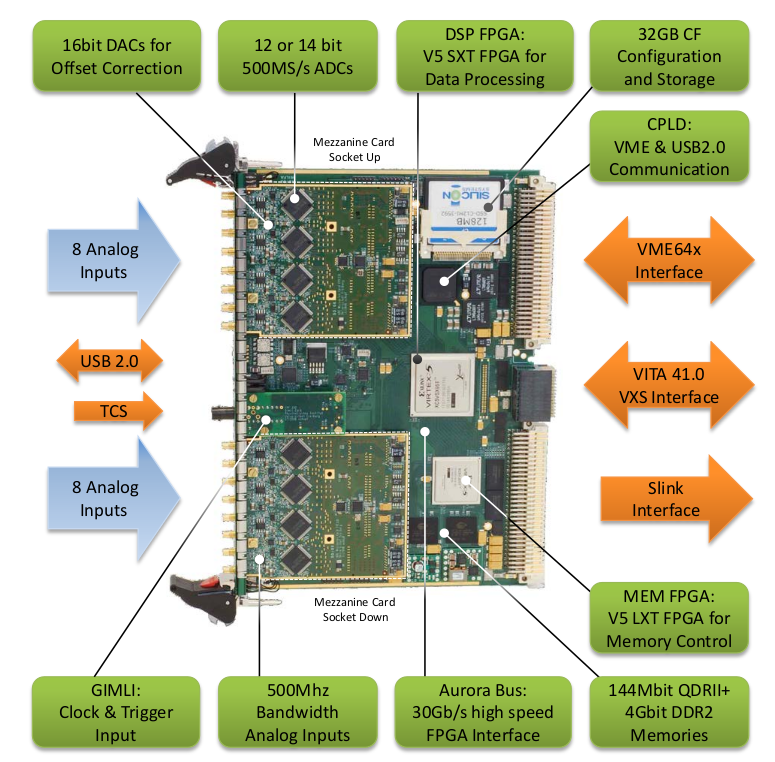
\includegraphics[width=1.\linewidth]{pictures/gandalf_overview.png}
	\label{fig:gandalf_overview}
	\caption{Overview of the Gandalf module equiped with Analog Mezzanin Cards (AMCs) and the fiber Gimli mezzanin card for clock an trigger input. The analog waveforms are digitized by the AMCs and the digitized data is processed by the DSP FPGA. The MEM FPGA handles the memory of the processed data, which can be transfered to a computer via the USB inteface on the front of the VME or S-Link interfaces on the backplane. \cite{herrmann}}
\end{figure}

\subsubsection{Input Mezzanin Cards}
The Gandalf module has two mezzanin card slots for input signals.
For these slots three different mezzanine cards were developed, \ac{amc}, \ac{dmc} and \ac{omc}.
First the latter two mezzanine cards are shortly presented for completeness but are not relevant for the work done in this thesis.

\paragraph{The \ac{dmc}} has 64 digital inputs. 
A picture of it is shown in \autoref{fig:dmc}.
Using either the LVDS or the LVPECL signal standard, one can use the DSP-\ac{fpga} logic for tasks like trigger decisions, time-to-digital conversion or pattern generators, to name a few.
By changing the direction of the input buffer on the \ac{dmc} \ac{pcb}, the 64 channels of the \ac{dmc} can be used as outputs intead of inputs.

\paragraph{The \ac{omc}} has four \SI{3.25}{\giga\bit\per\second} transceivers to receive digital informations, which can be further processed by the DSP-\ac{fpga}.
With this mezzanine card, the GANDALF can be used for example to merge data or as a concentrator.
A picture of a \ac{omc} is shown in \autoref{fig:omc}.

\paragraph{The \ac{amc}} is designed to digitize analog input signals.
For the digitization, eight \ac{adc} are used.
There are \ac{amc} with two different \ac{adc} available.
One is the \textit{ADS5463} with \SI{12}{\bit} and up to \SI{500}{\mega\sample\per\second} and the other is the \textit{ADS5474} which samples with up to \SI{400}{\mega\sample\per\second} at \SI{14}{\bit}.
The \ac{enob} of both \acp{adc} are \SI{10.4}{\bit} and \SI{11.2}{\bit} respectively.
Each \ac{amc} has eight SMC connectors for the inputs.
There are \ac{amc} operating in \textit{normal mode}, meaning each SMC connector is connected to one \ac{adc}, resulting in eight channels with up to \SI{500}{\mega\sample\per\second} or \SI{400}{\mega\sample\per\second} per \ac{amc}.
In order to increase the sample frequency, \ac{amc} which operate in the \textit{interleaved mode} were build.
On these \acp{amc} four inputs are connected to two \ac{adc}s each and therefore every second SMC connector is a dead end.
The clock signals which provide the sample tact for the two \acp{adc} of one channel have \SI{180}{\degree} phase offset in respect to each other.
By this the sample frequency is doubled to up to \SI{1}{\giga\sample\per\second} or \SI{800}{\mega\sample\per\second}, but the number of channels per \ac{amc} is reduced from eight to four.
The dynamic input range of the \ac{amc} is \SI{4.4}{\vpp} and can be shifted from the negative unipolar range \SIrange{-4.4}{0}{\volt} up to the bipolar range \SIrange{-2.2}{2.2}{\volt}.
This shifting is done by a \textit{AD5665R}, a \SI{16}{\bit} \ac{dac}.
The dynamic range was chosen because in the COMPASS experiment, for which the GANDALF was developed, negative voltage pulses created by \acp{pmt} needed to be digitized.
But because the used \acp{adc} expect positive differential signals, inverting operational amplifiers are used to change the polariy of the signal.
By changing the gain of the amplifiers one can decrease the input range and therefore increase the amplitude resolution.
The \acp{amc} used in this thesis are \SI{12}{\bit} \acp{amc} in the \textit{interleaved mode} and a dynamic range of \SI{2.2}{\vpp}.


\subsubsection{Usage of the GANDALF with \acp{sipm}}
In this work, the GANDALF was used to digitize the ouput signal of the \ac{emusic} \ac{asci}.
As mentioned in above in \autoref{sec:emusic} theses signals have a positive polarity.
But because the GANDALF was designed for the digitization and processing of negative voltage pulses created by a \ac{pmt}, this caused some problems.
Since after the inverting operational amplifiers in the GANDALF the \ac{sipm} signals have a negative polarity, the input voltage range needs to be chosen to be bipolar and around \SIrange{-1.1}{1.1}{\volt}.
In order to get this input range the baseline at \SI{0}{\volt} would need to be set to \SI{2047}{\adcu}.
For unknown reasons the programm which configeres the \acp{dac} to set the baseline to a \si{\adcu} value selectable by the user will set the baseline to a maximum of around \SI{1400}{\adcu}.
With $\frac{2.2}{2^12}\,\si{\volt\per\adcu} = \SI{0.537}{\milli\volt\per\adcu}$ the range of the inverted signal is \SI{1400}{\adcu} which corresponds to approximately \SI{752}{\milli\volt}.
Should this range be not enough, one needs to either try to find the source of the problem and fix it or decrease the amplification of the \ac{emusic} \ac{asic}.

The next problem regards the self-trigger of the GANDALF.
It functions via samples-over-threshold, the user can set a threshold and a number of consecutive samples which need to be over the threshold for the GANDALF to trigger an event.
Since after the inverting of the positive signals the signals have a negative polarity, the threshold needs to be set to a lower \si{\adcu} value than the baseline.
In addition to that the sample-over-threshold condition in the GANDALF firmware needed to be inverted to trigger if a number of consecutive samples are below the threshold.
The new firemware with the inverted trigger condition was tested and works as intended with the exception of one bug.
If the data rate from the GANDALF to the \ac{daq} computer exceeds the maximum possible data rate, \SI{20}{\mega\byte\per\second} in case of the USB inteface, incomplete events will be written down to disk.
This is most likely caused by a missing VHDL file that was not included in the new firmware and which would, incase the buffer of the GANDALF is completly filled, prevent the GANDALF to send incomplete events to the computer.
For the intended use of this bug should not be a problem, since the data rate is expected to be way below the possible \SI{20}{\mega\byte\per\second}.
